% !TeX spellcheck = en_US
%----------------------------------------------------------------------------------------
%	PACKAGES AND THEMES
%---------------------------------------------------------------------------------------
\documentclass{beamer}

% \DeclareMathOperator{\sinc}{sinc}
% \DeclareMathOperator{\si}{Si}
% \DeclareMathOperator{\sgn}{sgn}
% \DeclareMathOperator{\avg}{avg}
\usepackage[latin1]{inputenc} %Permite poner acentos directamente y e�es
\usepackage[spanish]{babel}
%\usepackage[caption=false,labelformat=simple]{subfig}
%\renewcommand{\thesubfigure}{(\alph{subfigure})}
\usepackage{psfrag}
\usepackage{graphicx} % Allows including images
\usepackage{booktabs} % Allows the use of \toprule, \midrule and \bottomrule in tables
\usepackage{textpos}
\usepackage{pgf}  
\usepackage{array}
\usepackage{float} 
\usepackage{appendixnumberbeamer}
% Add total frame count to slides, optional. From Stefan,
% http://www.latex-community.org/forum/viewtopic.php?f=4&t=2173
\usepackage{sansmathaccent}
%\pdfmapfile{+sansmathaccent.map}
\usepackage{textcomp}  %trademark symbol

\usepackage{amsmath}
\usepackage{amssymb}
\usepackage{cite}
\usepackage{subcaption}
%\usepackage[dvipsnames,table,xcdraw]{xcolor}

\usepackage{caption}
\usepackage{amsthm}
\usepackage{soul}
\usepackage{mathtools}% para ecuacion apendice
\usepackage{float}%para subfigures
%\usepackage{gensymb} % para degree symbol
%\usepackage[scr]{rsfso} %para Laplace
\usepackage{hhline}



\expandafter\def\expandafter\insertshorttitle\expandafter{%
	\insertshorttitle\hfill\insertframenumber\,/\,\inserttotalframenumber}


\mode<presentation> {
	
	% The Beamer class comes with a number of default slide themes
	% which change the colors and layouts of slides. Below this is a list
	% of all the themes, uncomment each in turn to see what they look like.
	
	%\usetheme{default}
	\usetheme{AnnArbor}
	%\usetheme{Antibes}
	%\usetheme{Bergen}
	%\usetheme{Berkeley}
	%\usetheme{Berlin}
	%\usetheme{Boadilla}
	%\usetheme{CambridgeUS}
	%\usetheme{Copenhagen}
	%\usetheme{Darmstadt}
	%\usetheme{Dresden}
	%\usetheme{Frankfurt}
	%\usetheme{Goettingen}
	%\usetheme{Hannover}
	%\usetheme{Ilmenau}
	%%\usetheme{JuanLesPins}
	%\usetheme{Luebeck}
	%\usetheme{Madrid}
	%\usetheme{Malmoe}
	%\usetheme{Marburg}
	%\usetheme{Montpellier}
	%\usetheme{PaloAlto}
	%\usetheme{Pittsburgh}
	%\usetheme{Rochester}
	%\usetheme{Singapore}
	%\usetheme{Szeged}
	%\usetheme{Warsaw}
	
	% As well as themes, the Beamer class has a number of color themes
	% for any slide theme. Uncomment each of these in turn to see how it
	% changes the colors of your current slide theme.
	
	%\usecolortheme{albatross}
	%\usecolortheme{beaver}
	%\usecolortheme{beetle}
	%\usecolortheme{crane}
	%\usecolortheme{dolphin}
	%\usecolortheme{dove}
	%\usecolortheme{fly}
	%\usecolortheme{lily}
	%\usecolortheme{orchid}
	%\usecolortheme{rose}
	%\usecolortheme{seagull}
	%\usecolortheme{seahorse}
	\usecolortheme{whale}
	%\usecolortheme{wolverine}
	
	% \setbeamertemplate{footline} % To remove the footer line in all slides uncomment this line
	\setbeamertemplate{footline}[frame number] % To replace the footer line in all slides with a simple slide count uncomment this line
	
	%\setbeamertemplate{navigation symbols}{} % To remove the navigation symbols from the bottom of all slides uncomment this line
}



\newenvironment<>{ferblock}[2][0.9\textwidth]{
	\begin{center}
		\vskip-6cm
		\begin{minipage}{#1}
			\setlength{\textwidth}{#1}
			\begin{actionenv}#3
				\def\insertblocktitle{#2}
				\par
				%\setbeamercolor{block title}{fg=white,bg=orange!20!black}%bg=background, fg= foreground
				\setbeamercolor{block body}{fg=black,bg=olive!20}%bg=background, fg= foreground
				\setbeamercolor{block title}{fg=blue!10,bg=orange!20!blue}			
				\usebeamertemplate{block begin}}
			{\par 
				\usebeamertemplate{block end}
			\end{actionenv}
		\end{minipage}
\end{center}} 



%----------------------------------------------------------------------------------------
%	TITLE PAGE
%----------------------------------------------------------------------------------------

\title{End to end developments for the Multipurpose Interferometer Array Pathfinder from the IAR Electronics Laboratory.}
%\subtitle{Proyecto MIA}

\author{Hugo Command, Juan M. Gonzalez, 
	Gast�n Valdez}


\institute[IAR] % Your institution as it will appear on the bottom of every slide, may be shorthand to save space
{Instituto Argenitno de Radioastronom�a (IAR) \\
	Camino Gral. Belgrano Km 40, Berazategui, Argentina\\ % Your institution for the title page
	\medskip
	\textit{hcommand@iar.unlp.edu.ar; jmgonzalez@iar.unlp.edu.ar;gvaldez@iar.unlp.edu.ar} \\ % Your email address
	\medskip
	
\includegraphics[width=8cm,keepaspectratio]{Figuras/logplantillatransparente.eps} \medskip \hspace{0.3cm}\\
	%\includegraphics[width=1cm,height=1cm,keepaspectratio]{logo_uns_nuevo1.eps}\\
	
}
\date{} % Date, can be changed to a custom date


\setbeamercolor*{frametitle}{bg=blue!20}


\begin{document}
	
	\begin{frame}
		\titlepage % Print the title page as the first slide
	\end{frame}
	
	%LOGOS EN TODAS LAS FILMINAS
	\addtobeamertemplate{frametitle}{}{%
		\begin{textblock*}{100mm}(.85\textwidth,-0.82cm)
			\hspace{0.5cm}
			
\includegraphics[width=0.75cm,keepaspectratio]{Figuras/logoiar_2019.eps} %\hspace{0.1cm}
			%\includegraphics[width=0.7cm,height=0.7cm,keepaspectratio]{logo_uns_nuevo1.eps}
	\end{textblock*}}
	
	
	%\section{Descripci�n del sistema}
	\section{Front-End}
	
	\begin{frame}
		\frametitle{Front-End}
		
		%\begin{figure}
		%	\centering
		%	
\includegraphics[width=0.8\columnwidth]{Figuras/logplantillatransparente.eps}
		%%	\caption{Inversor conectado a la red.}
		%\end{figure}
	\end{frame}
	
	
	\section{Back-End}
	
	\frametitle{Back-End}
	
	
	
	\begin{frame}
		\frametitle{Back-End}
		
		The Smart Network ADC Processor (SNAP) board consists of three HMCAD1511 8-bit analogue to digital converters (ADCs), capable of sampling 500 MHz for three 	signals per board. 
		
		The ADCs are connected to a Kintex-7 160T field-programmable gate array (FPGA), 
		
		with an associated dual
		10 GbE port. 
		
		Each SNAP board is controlled via Raspberry Pi, which interacts with a controlling PC over ethernet via a series of PYTHON scripts.
		
	\end{frame}
	
	\begin{frame}
		\frametitle{System features}
		
		
		\begin{center}
			\begin{tabular}{||c | c||} 
				\hline
				\textbf{Parameter} & \textbf{Value}  \\ [0.5ex] 
				\hline\hline
				Sample Frequency & 500 MHz  \\ 
				\hline
				BW & 250 MHz  \\
				\hline
				Centered Frequency & 1325 MHz  \\
				\hline
				Board & SNAP (Casper) \\[1ex] 
				\hline
				Development environment& Casper Toolflow \\[1ex] 
				\hline
				
			\end{tabular}
		\end{center}
		
		
	\end{frame}
	
	
	\begin{frame}
		%\frametitle{}
		\begin{figure}
			\centering
			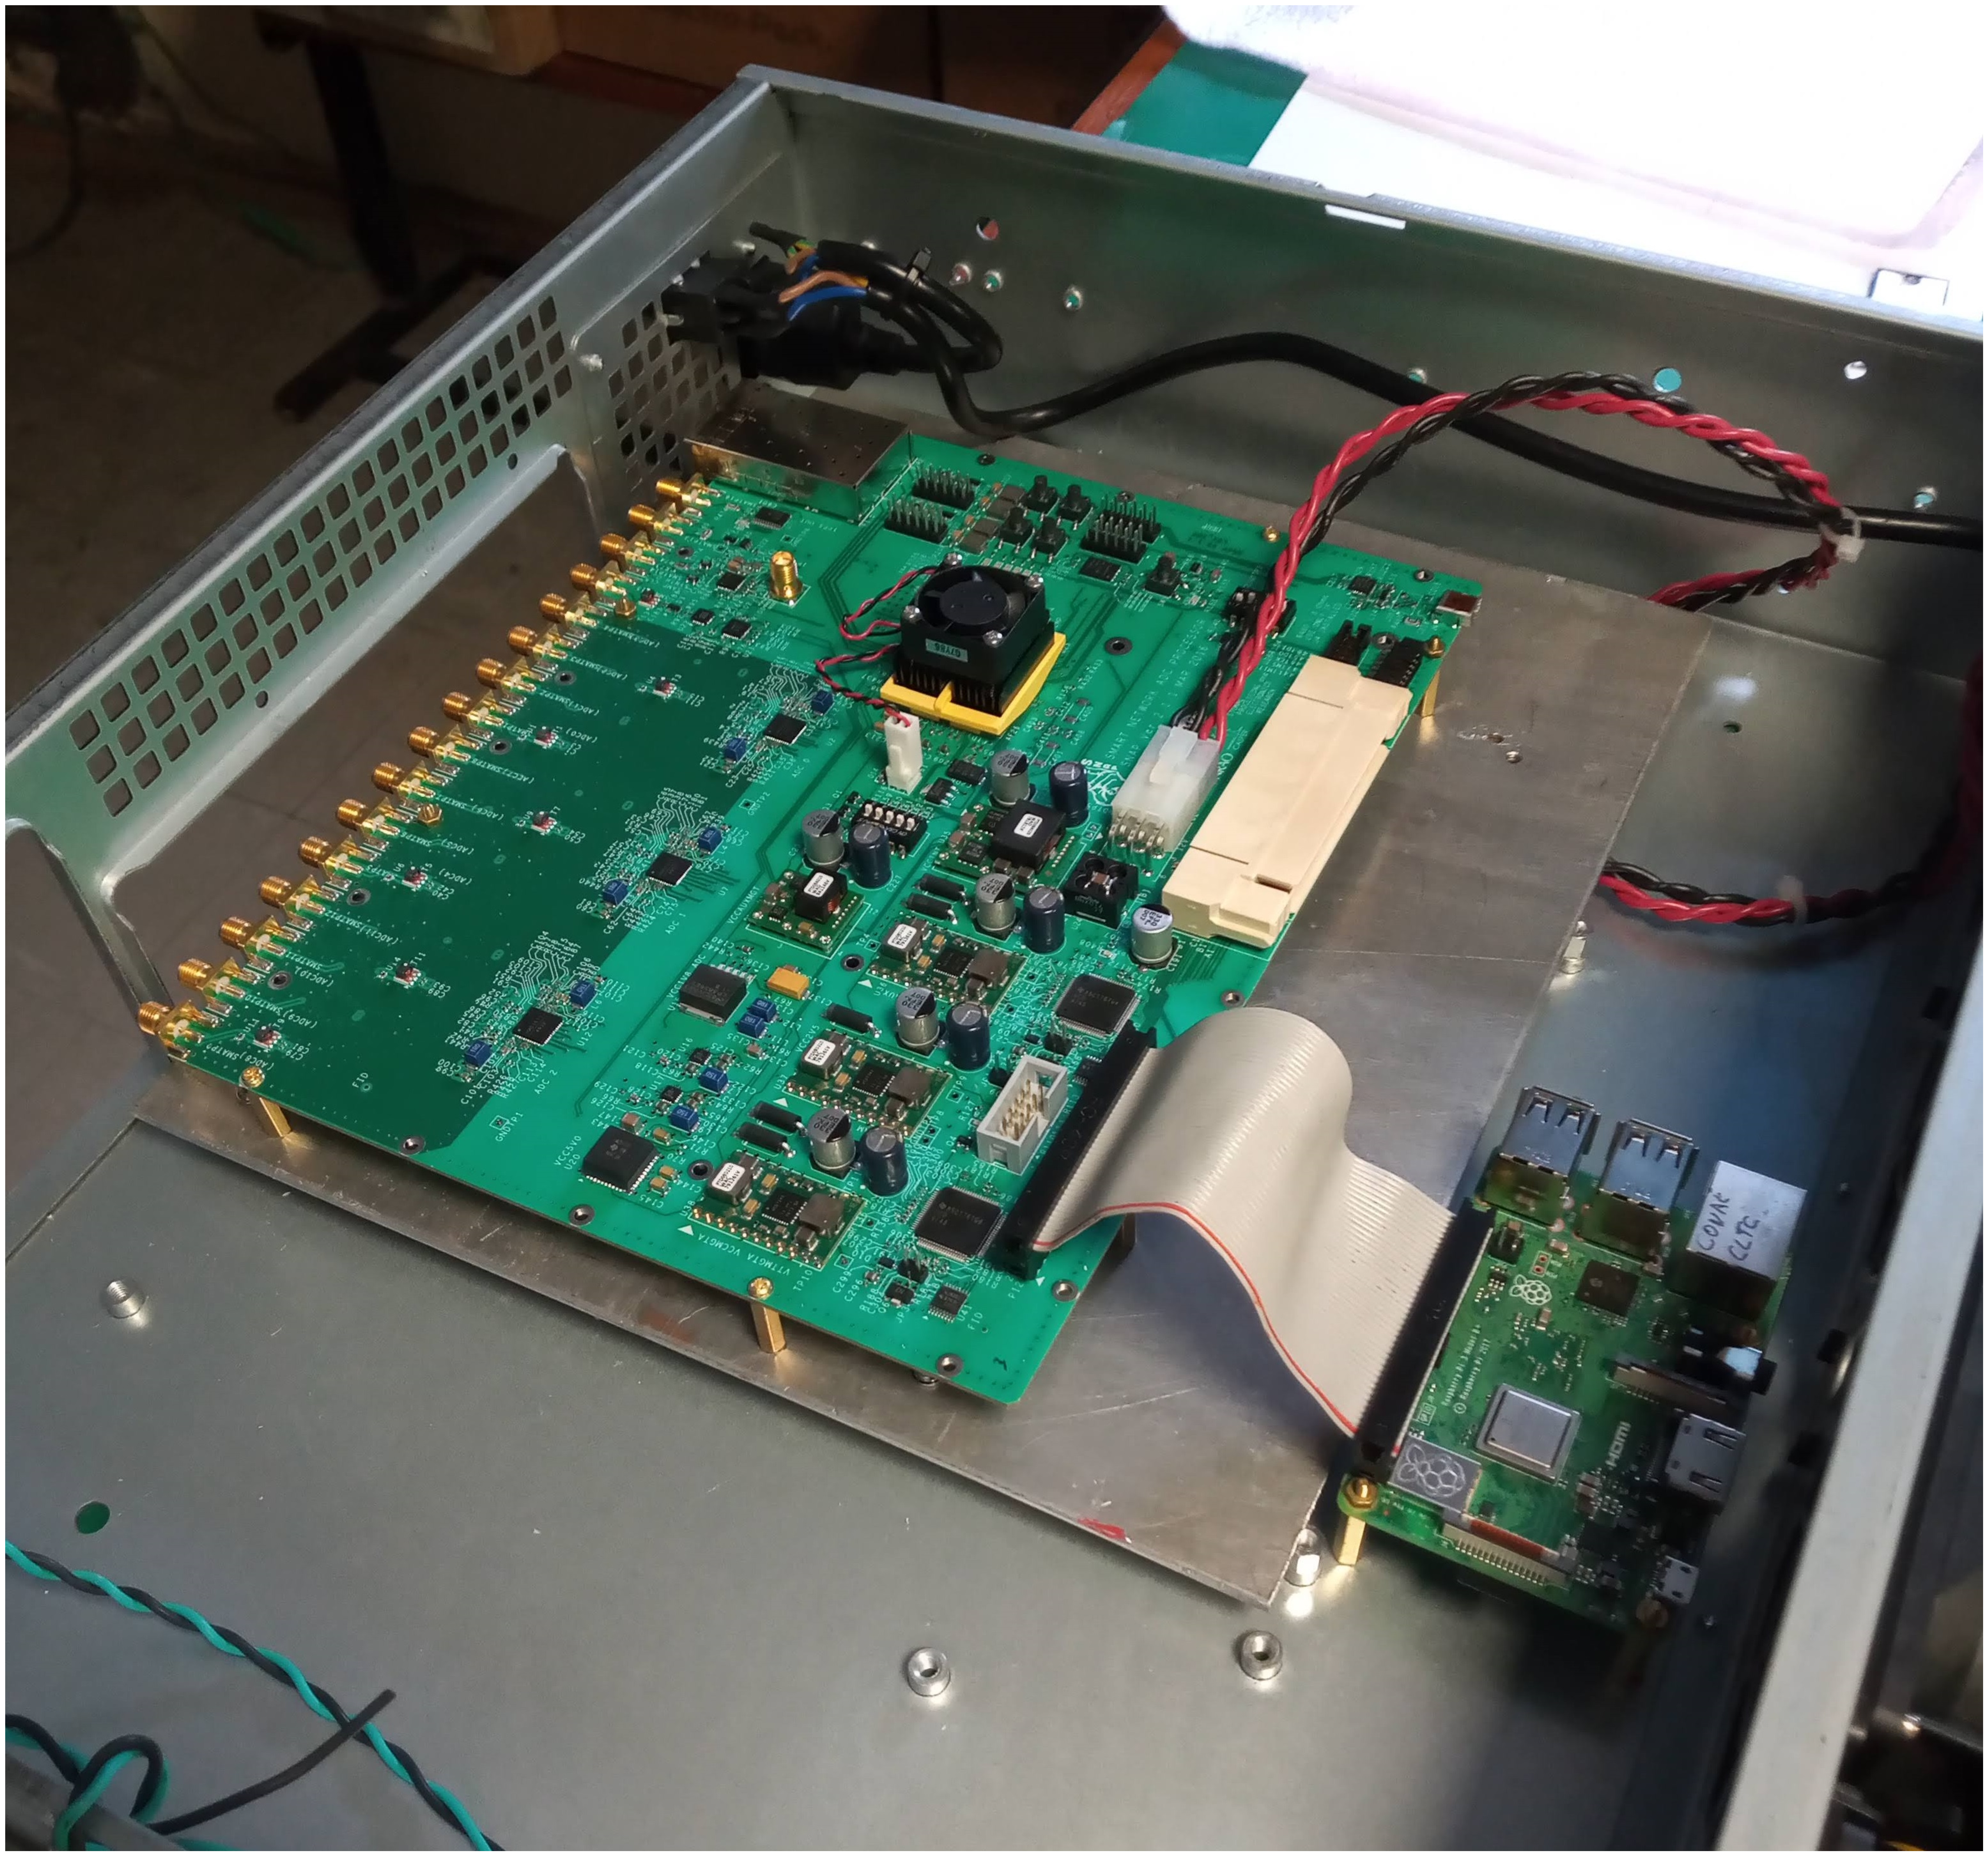
\includegraphics[width=0.4\columnwidth]{Figuras/snap1.eps}
			%	\caption{Inversor conectado a la red.}
		\end{figure}
		
		\begin{figure}
			\centering
			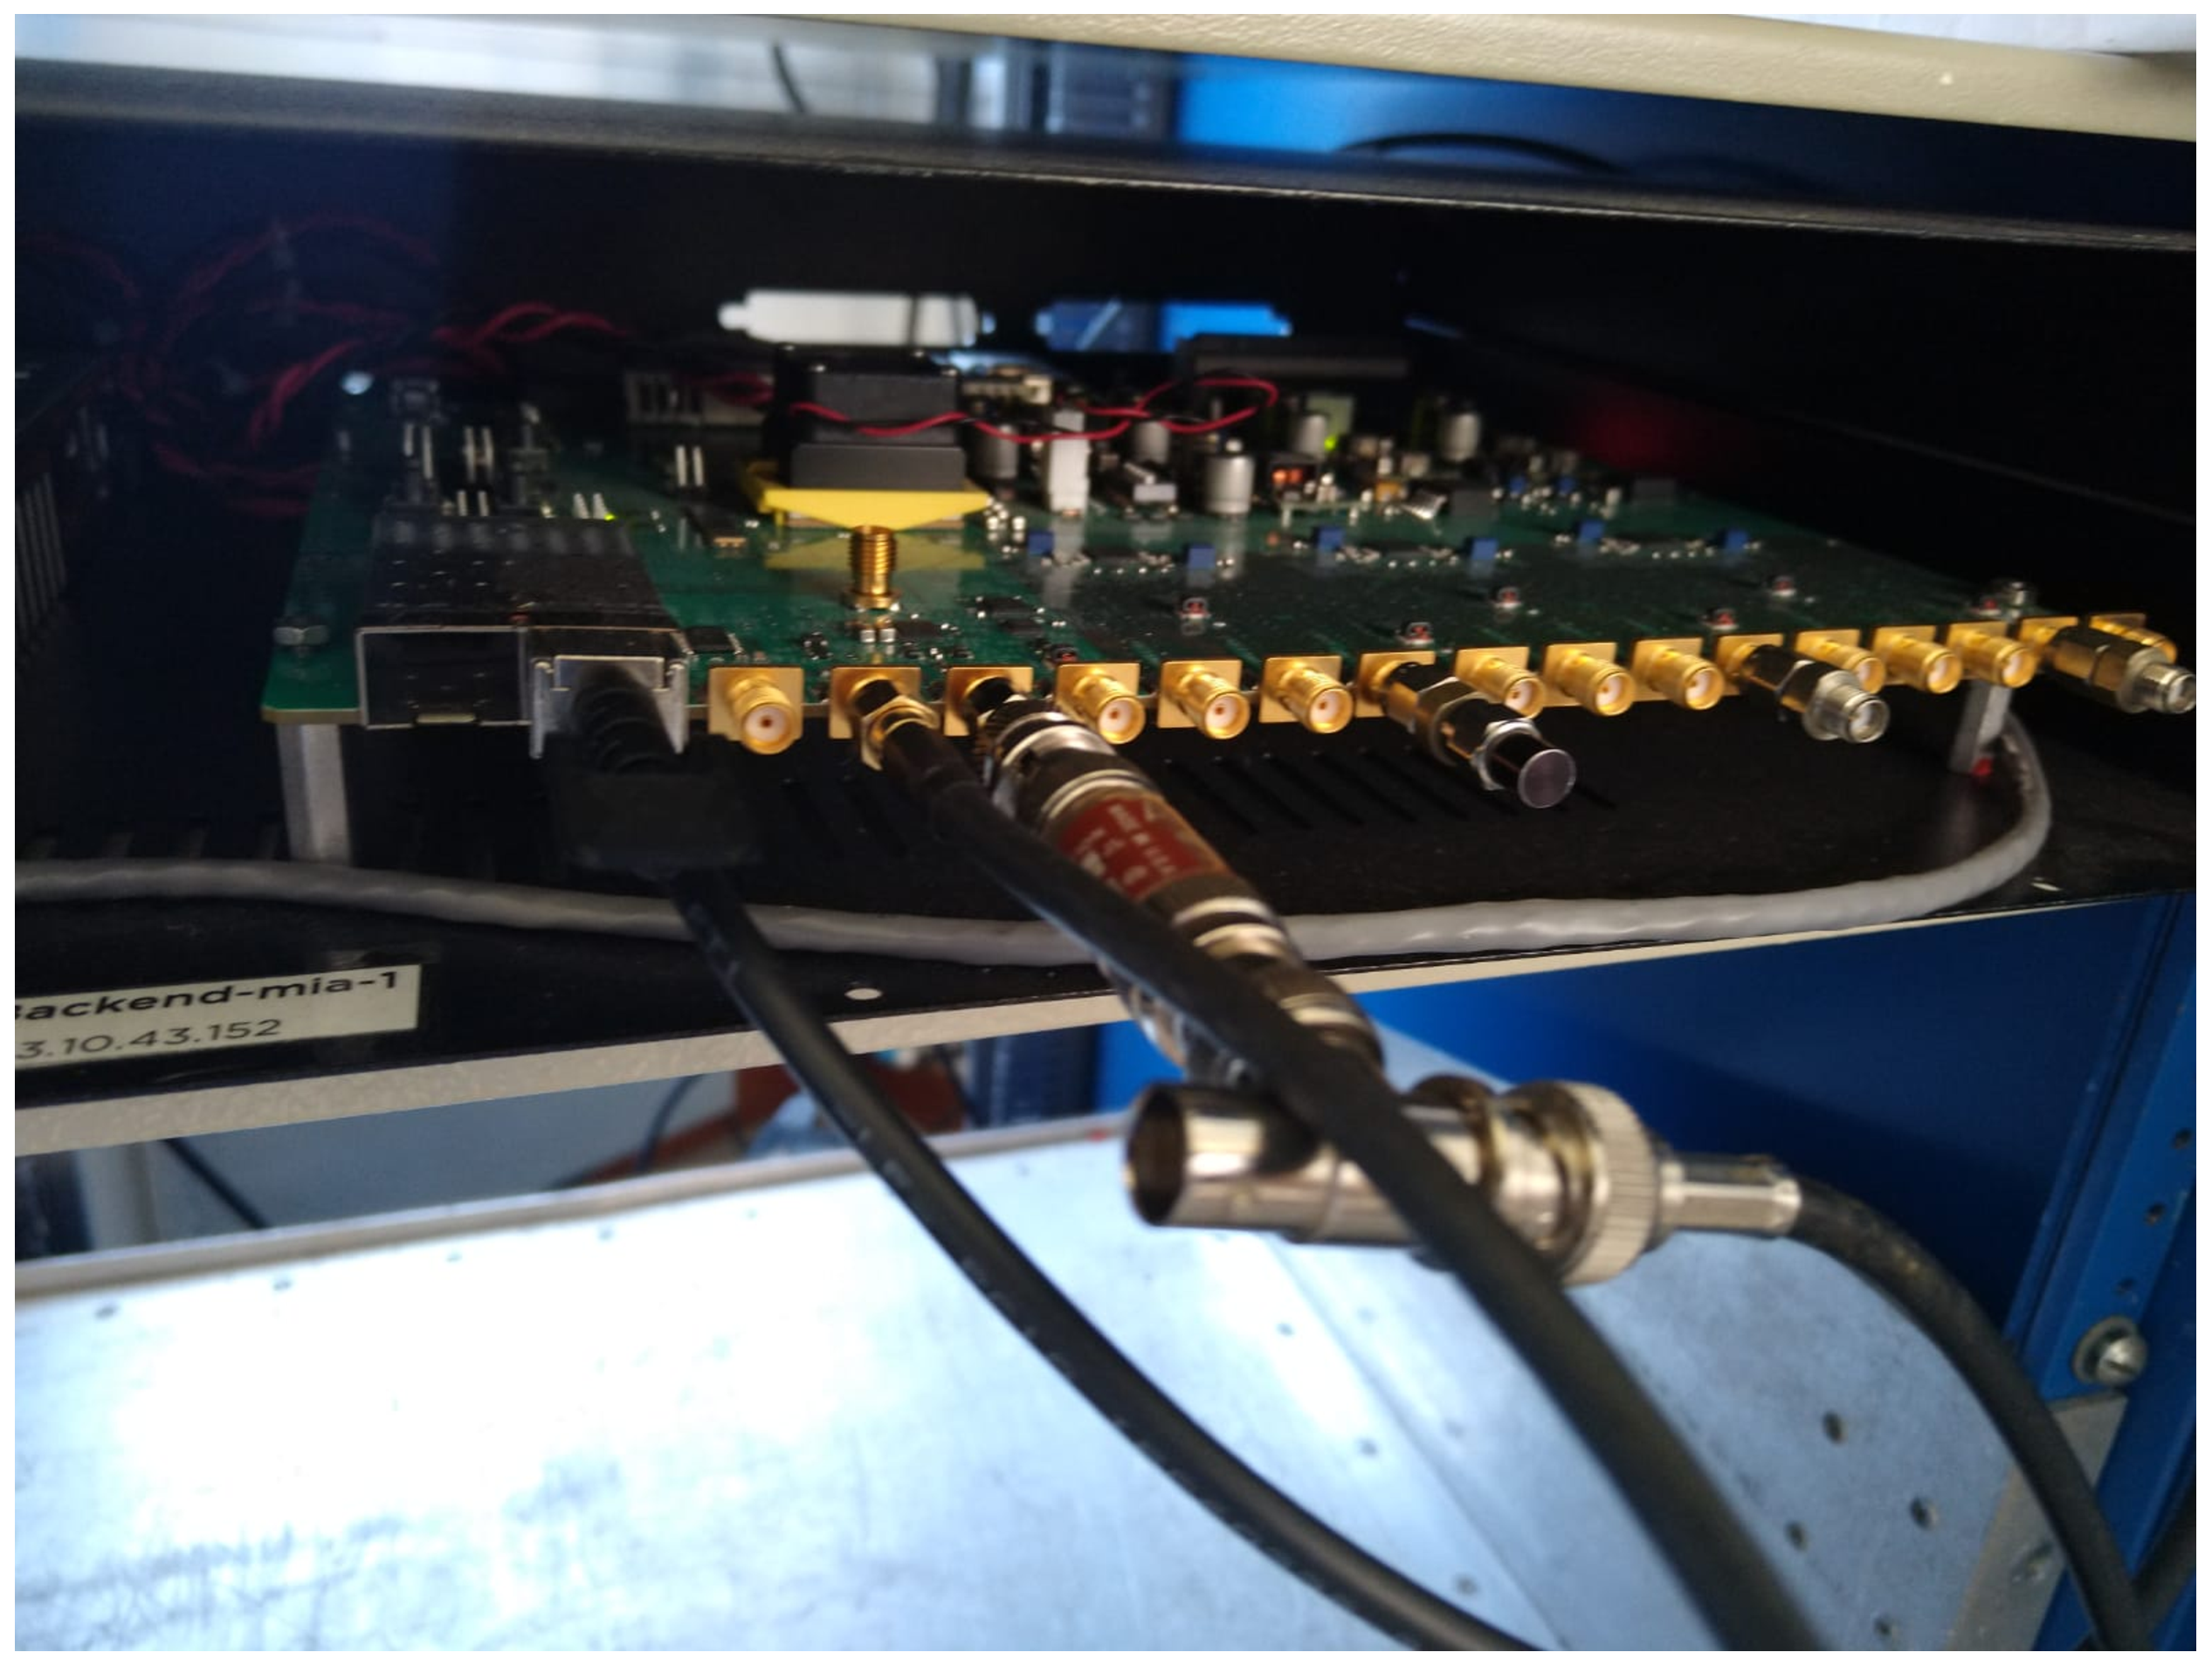
\includegraphics[width=0.4\columnwidth]{Figuras/snap2.eps}
			%	\caption{Inversor conectado a la red.}
		\end{figure}
		
	\end{frame}
	
	
	\begin{frame}
		\frametitle{Back-End Module}	
		\begin{figure}
			\centering
			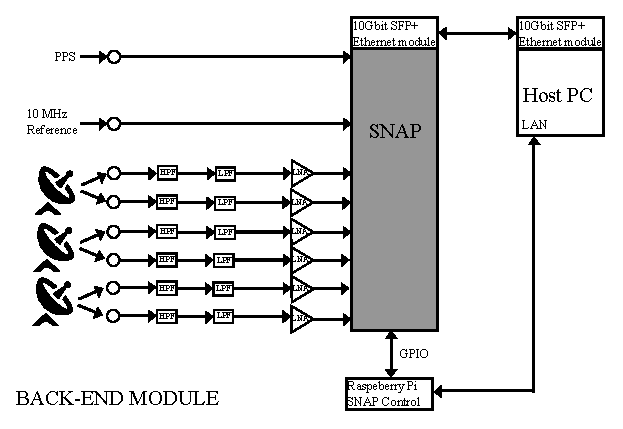
\includegraphics[width=0.8\columnwidth]{Figuras/diagrama_back_end_6ch.eps}
			%	\caption{Inversor conectado a la red.}
		\end{figure}
	\end{frame}
	
	
	\begin{frame}
		\frametitle{Spectrometer for system verification}	
		\begin{figure}
			\centering
			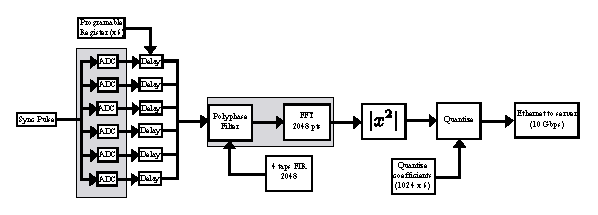
\includegraphics[width=1\columnwidth,,keepaspectratio]{Figuras/FPGA_internal.eps}
			%	\caption{Inversor conectado a la red.}
		\end{figure}
	\end{frame}
	
	\section{Position Control}
	
	\begin{frame}
		\frametitle{Position Control}
		\Large{Design based open hardware and open software}
		\begin{itemize}
			\item Python: Generate path trajectories stars for testing system.
			\item CMake : Tool for compile project and independent system build.
			\item Languaje programming: C/C++ and Python   
			\item Ceedling: Framework for testing embebbed systems. 
			%		\item Git and Github: TBD
		\end{itemize}
		\begin{figure}
			\centering
			
\includegraphics[width=1\columnwidth]{soft_figures/logos.eps}
			%	\caption{Inversor conectado a la red.}
		\end{figure}
		
		
		
	\end{frame}
	
	\begin{frame}
		\frametitle{Position Control}
		The software design using architecture of layers. 
		\begin{figure}
			\centering
			\includegraphics[width=1\columnwidth]{soft_figures/soft_layer.eps}
		\end{figure}
		
		
	\end{frame}
	
	
%	\begin{frame}
%		\frametitle{Position Control}
%		
%		\begin{itemize}
%			\item layer interface: Interface betwen hardware and software controller position. 
%			\begin{itemize}
%				\item web server: TBD
%				\item gpredict\_sockets: protocol adapter to python(in process, actually format code using C) 
%				\item stellarium\_sockets: protocol adapter to python(in process, actually format code using C) 
%				\item API\_sockets: terminal interface using ssh or sockets commands, depends gerency projects and antenna operators. 
%				
%			\end{itemize}
%			\item app web: processes data between interface and database, manages connections to hardware
%			\item management\_app: it gets data from the sensors and information from the control, and sends it to the app layer. It also manages GPIO's ports and saves a list of radio sources to track.
%			\item controller: manage control hardware and sensors
%			
%		\end{itemize}
%		
%	\end{frame}
%	
	
	
	\begin{frame}
		\frametitle{Position Control}
		The controller layer obtains environmental parameters and applies the control algorithm. A distributed system has been created using Raspberry Pi Pico (RP2040 microcontroller). 
		
		\begin{figure}
			\centering
			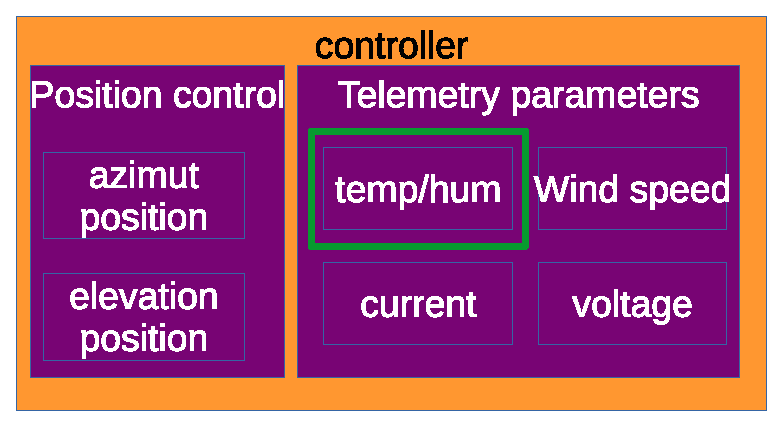
\includegraphics[width=1\columnwidth]{soft_figures/contoller_layer.eps}
		\end{figure}
		Position controller are identical for each axis.
	\end{frame}
	
	
	
	\begin{frame}
		\frametitle{Position Control}
	 Example reports generate automatically using ceedling (reports for Code Coverage using Ceedling). 
	
		\begin{figure}
			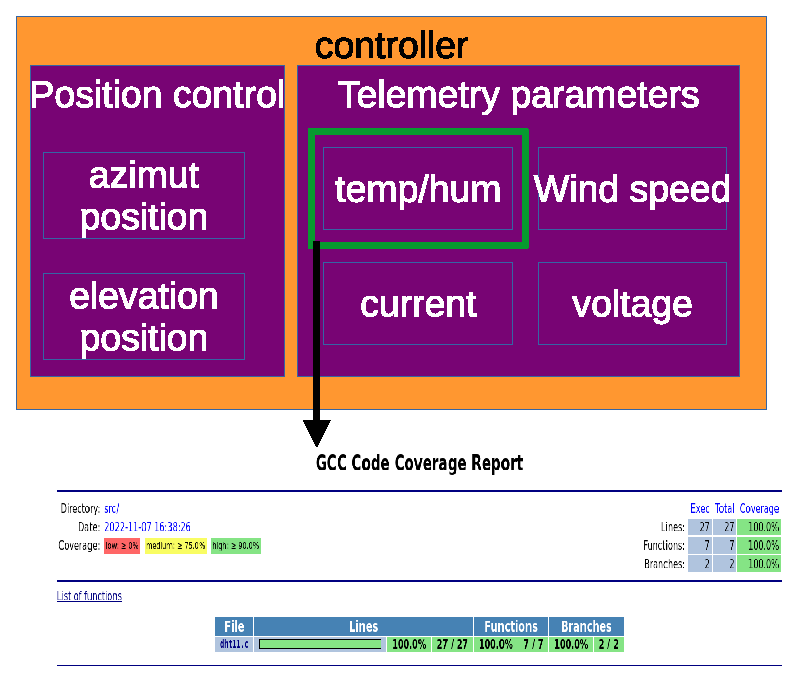
\includegraphics[width=\textwidth,height=6cm]{soft_figures/gcov_reports.eps}
		\end{figure}
	\end{frame}
	
	
\begin{frame}
	\frametitle{Position Control}
	Connect antenna pointing to Gpredict and Stellarium software. 	Compute sidereal time using eight 8 bits microcontroller for a test and error obtained is 0.07S .RP2040 is a 32 bits it is expected to improve the error. Testbench using astropy and algoritms for a calculus sidereal time.   
	\begin{figure}
		\vspace{-0.8cm}
		\includegraphics[width=\textwidth,height=6cm]{soft_figures/gpredict_stellarium_reports.eps}
	\end{figure}
\end{frame}






\begin{frame}
	\frametitle{Position Control}




\end{frame}



	
	
	\section{Conclusiones}
	\begin{frame}
		\frametitle{Conclusiones}
		
		\begin{enumerate}
			
			\onslide<1->\item C1 
			\onslide<2->\item C2
			\onslide<3->\item C3
			\onslide<4->\item C4
		\end{enumerate}
		
		
	\end{frame}
	
	
	\begin{frame}
		\begin{center}
			\textbf{Questions $\cdots$}
		\end{center}
	\end{frame}
	
	
\end{document} 